% Created 2022-05-21 sáb 15:30
% Intended LaTeX compiler: pdflatex
\documentclass[presentation]{beamer}
\usepackage[utf8]{inputenc}
\usepackage[T1]{fontenc}
\usepackage{graphicx}
\usepackage{grffile}
\usepackage{longtable}
\usepackage{wrapfig}
\usepackage{rotating}
\usepackage[normalem]{ulem}
\usepackage{amsmath}
\usepackage{textcomp}
\usepackage{amssymb}
\usepackage{capt-of}
\usepackage{hyperref}
\logo{\includegraphics[height=0.5cm]{./assets/lOGO-HORIZONTAL-KONRAD-COLOR.jpg}}
\usetheme[height=20pt]{Rochester}
\author{Jonatan Ahumada}
\date{\today}
\title{Modelo de literariedad basado en la lingüistica de Roman Jakobson}
\subtitle{Fundación Universitaria Konrad Lorenz}
\hypersetup{
 pdfauthor={Jonatan Ahumada},
 pdftitle={Modelo de literariedad basado en la lingüistica de Roman Jakobson},
 pdfkeywords={},
 pdfsubject={},
 pdfcreator={Emacs 27.2 (Org mode 9.4.4)}, 
 pdflang={Spanish}}
\begin{document}

\maketitle
\begin{frame}{Outline}
\tableofcontents
\end{frame}



\section{Introducción}
\label{sec:orge383d3e}

\begin{frame}[label={sec:org2c35e8a}]{¿Qué es \emph{literariedad}?}
Es una presunta \emph{característica} que distingue un texto literario de
otro no literario.

Por ejemplo:

\begin{itemize}
\item Manual de un carro vs. un poema de Jose Asunción Silva (fácil)
\item Artículo periodístico  vs. cuento corto  (normal)
\item \emph{50 sombras de Gray} vs. \emph{Ulysses} (difícil)
\end{itemize}
\end{frame}


\begin{frame}[label={sec:org1abb8a0}]{Antecedentes: Los clásicos}
En los estudios clásicos, se encuentran teorías acerca de qué constituye
un texto 'poético' o una buena 'narración'.

\begin{itemize}
\item Fedro, Platón
\item Póetica, Aristóteles
\item Carta a los pisones, Horacio
\end{itemize}

Sin embargo, el enfoque que toman estos autores no es \alert{metódico} o \alert{sistemático}
\end{frame}

\begin{frame}[label={sec:orga721ddf}]{Antecedentes: la linguística estructural}
En el siglo 20, Ferdinand de Saussure fundó la linguística general
(también llamada estructural). Se considera al fenómeno del
lenguaje como una estructura compuesta de varios componentes
interdependientes, pero identificables.
\end{frame}


\begin{frame}[label={sec:org1d6e7f7}]{Antecedentes: Roman Jakobson}
\begin{columns}
\begin{column}{0.48\columnwidth}
Roman Jakobson fue un lingüista ruso americano. Se considera una
figura clave tanto en movimiento del \emph{formalismo ruso}, así como
en el \emph{estructuralista}.  La lingüística de Jakobson se basa en
los postulados de la lingüistica de Saussure, \alert{pero} propuso una
crítica a las ideas de Saussure.
\end{column}


\begin{column}{0.48\columnwidth}
\begin{block}{Cita}
\begin{quote}
The fundamental role which these two operations play in language
was clearly realized by Ferdinand de Saussure. Yet of the two
varieties of combination-concurrence and concatenation-it was only
the latter, the temporal sequence, which was recognized by the
Geneva linguist. 
\cite[99]{jakobson1956two}
\end{quote}
\end{block}
\end{column}
\end{columns}
\end{frame}




\begin{frame}[label={sec:orgd2898be}]{La pregunta}
\begin{block}{}
   ¿Cómo medir
   computarizadamente la /literariedad/ de un texto según el marco de la
   lingüística de Jakobson?
\end{block}
\end{frame}


\section{Objetivos}
\label{sec:org20eba3d}
\begin{frame}[label={sec:org1916615}]{General}
   \begin{block}{General}

Diseñar e implementar un modelo que, dado un corpus de texto, produzca
   indicadores para el concepto de /literariedad/ que plantea Roman Jakobson.
     \end{block}
\end{frame}

\begin{frame}[label={sec:org89d5253}]{Específicos}
\begin{enumerate}
\item Construir el corpus necesario para representar el \emph{eje sincrónico}.
\item Diseñar e implementar el algoritmo para calcular la \emph{metáfora} sobre un corpus.
\item Diseñar e implementar algoritmo para calcular la \emph{metonimia} sobre un corpus.
\item Seleccionar y unir los textos que serán procesados (corpus objetivo) por el algoritmo.
\item Correr el algoritmo sobre los corpus objetivo.
\item Evaluar el algoritmo de manera cuantitativa y cualitativa.
\end{enumerate}
\end{frame}

\begin{frame}[label={sec:org70c29be}]{Alcance}
\begin{enumerate}
\item Modelos \alert{naive}

\item Corpus de acceso libre (Brown Corpus)

\item Herramientas 'básicas' de NLP. (no Machine Learning)
\end{enumerate}
\end{frame}

\section{Marco teórico y referencial}
\label{sec:org12cebd7}

\begin{frame}[label={sec:org66050c6}]{Introducción a metáfora y metonimia}
\begin{columns}
\begin{column}{0.48\columnwidth}
 \begin{figure}
 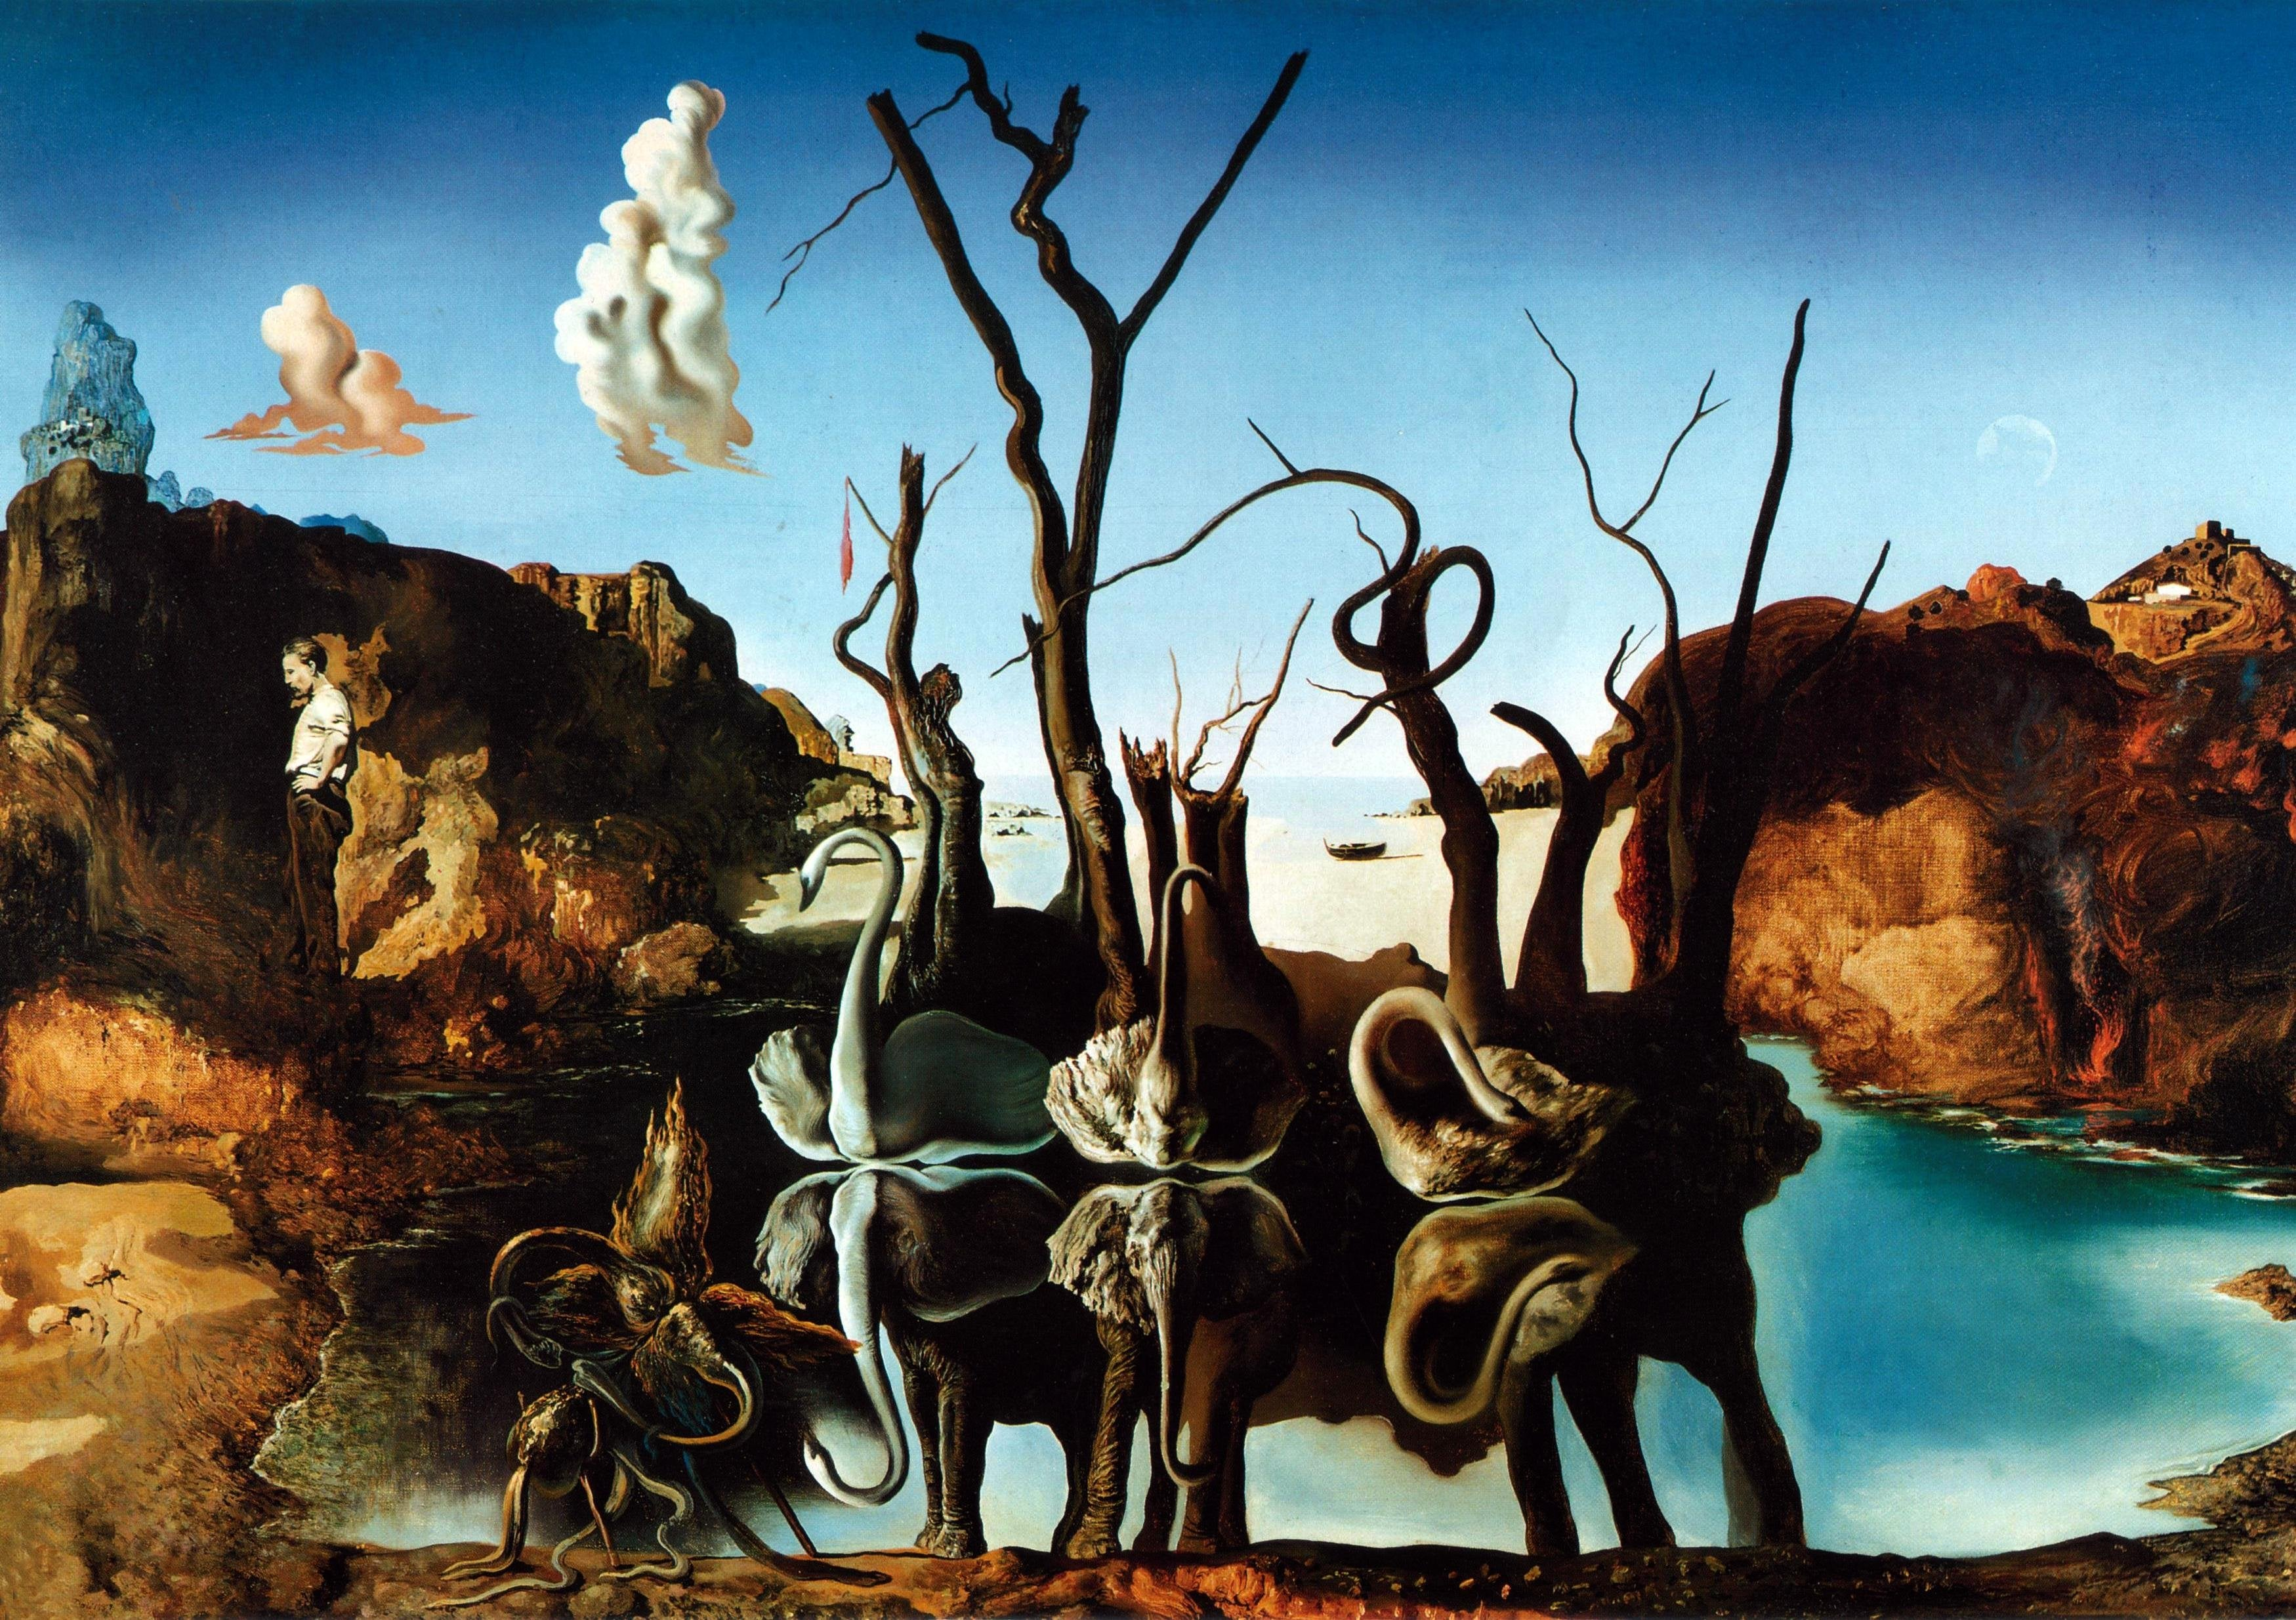
\includegraphics[width=\textwidth]{./assets/arte_dali.jpg}
\caption{\emph{Cisnes reflejando elefantes} de Salvador Dalí}
 \end{figure}
\end{column}

\begin{column}{0.48\columnwidth}
\begin{figure}
    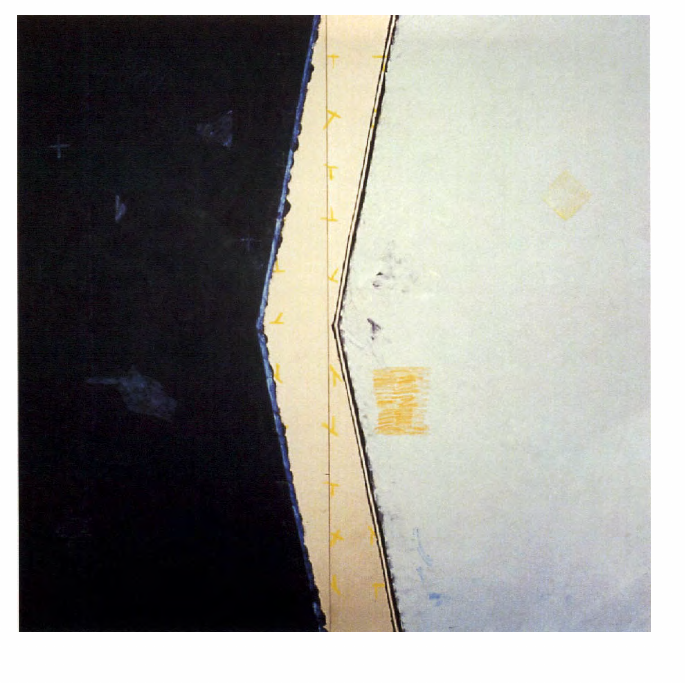
\includegraphics[width=\textwidth]{./assets/arte_green.png}
\caption{\emph{9 grados} de Denise Green}
 \end{figure}
\end{column}
\end{columns}
\end{frame}

\begin{frame}[label={sec:org4f06d5c}]{Metáfora y metonimia}
\begin{columns}
\begin{column}{0.48\columnwidth}
\begin{figure}
    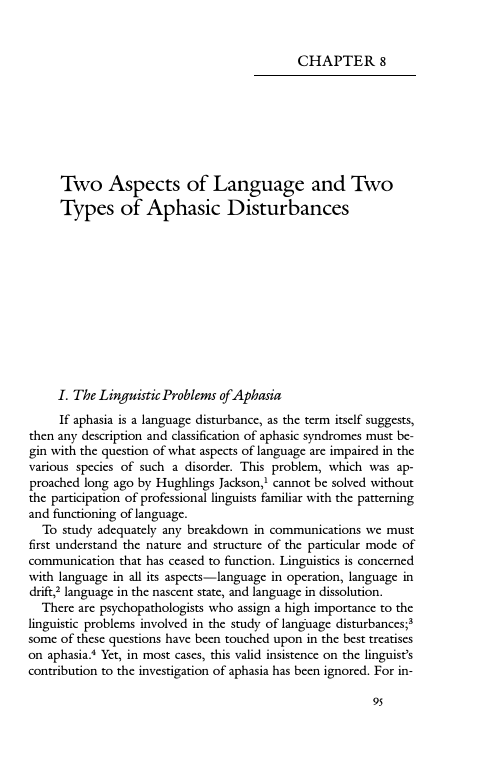
\includegraphics[width=\textwidth]{./assets/cover_two_aspects.png}
\caption{\emph{9 grados} de Denise Green}
 \end{figure}
\end{column}

\begin{column}{0.48\columnwidth}
\tiny
   \begin{block}{Combinación/Metonimia}
Any linguistic sign involves two modes of arrangement:
Any sign is made up of constituent signs and/or
occurs only in combination with other signs. This means that any lin­
guistic unit at one and the same time serves as a context for simpler
units and/or finds its own context in a more complex linguistic unit.

   \end{block}

   \begin{block}{Selección/Metáfora}
A selection between alternatives implies the possibility
of substituting one for the other, equivalent in one respect and differ­
ent in another. Actually, selection and substitution are two faces of the
same operation.


   \end{block}

\normal
\end{column}
\end{columns}
\end{frame}
\section{Diseño Metodológico}
\label{sec:orge7f1839}
\begin{frame}[label={sec:org7a72104}]{Metodología}
  \begin{figure}
   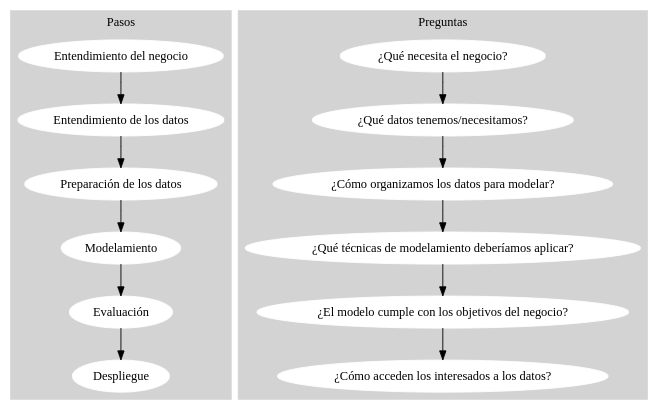
\includegraphics[width=\textwidth]{./assets/metodologia.png}

\end{figure}
\end{frame}

\begin{frame}[label={sec:orga7a4ca7}]{Entendimiento del negocio}
Cada algoritmo recibe un mensaje  \(m\) de entrada con:
\begin{block}{Entrada}
\begin{itemize}
\item cadena de cualquier longitud
\item sin POS
\item sin set de entrenamiento
\end{itemize}
\end{block}
produce:

\begin{block}{Salida}
\begin{itemize}
\item  Un valor continuo para dicho mensaje (no es categórico)
\item  Entre más alto el valor, más fuerte es esa característica (metáfora y/o metonímia)
\end{itemize}
\end{block}
\end{frame}

\begin{frame}[label={sec:orgd5b44b6}]{Usos}
  \begin{figure}
   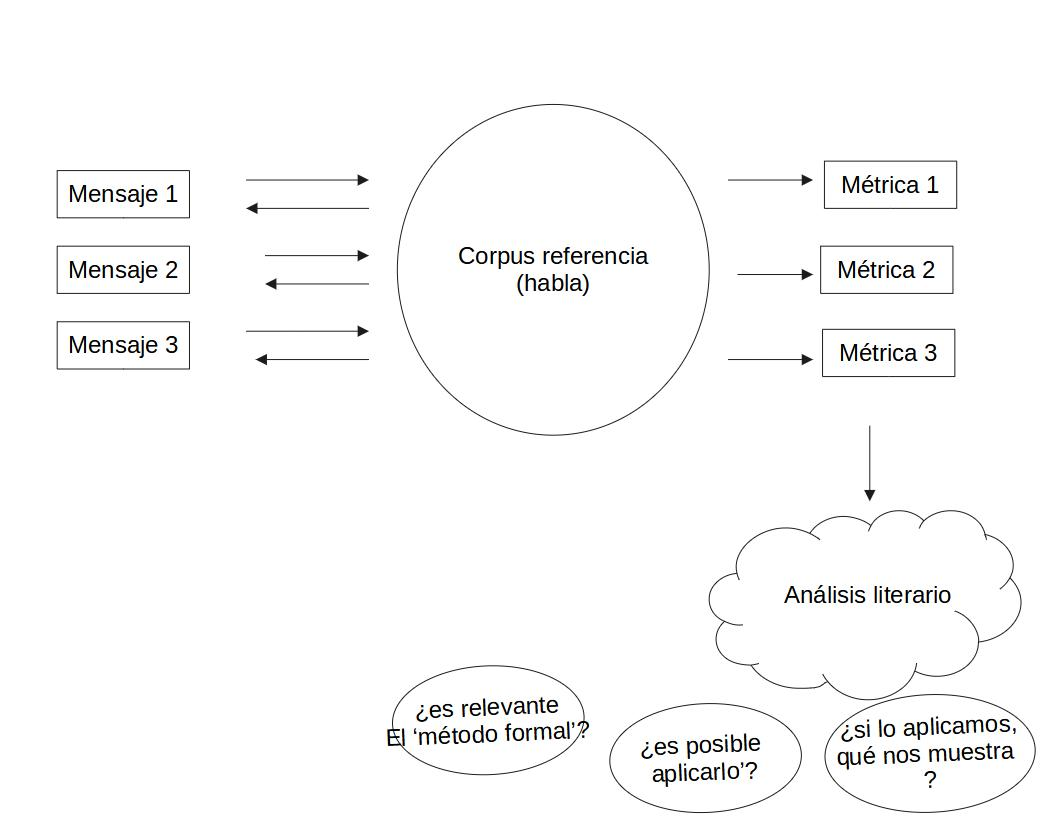
\includegraphics[width=\textwidth]{./assets/posibles_usos.jpg}

\end{figure}
\end{frame}


\begin{frame}[label={sec:org215656d}]{Usuarios}
  \begin{figure}
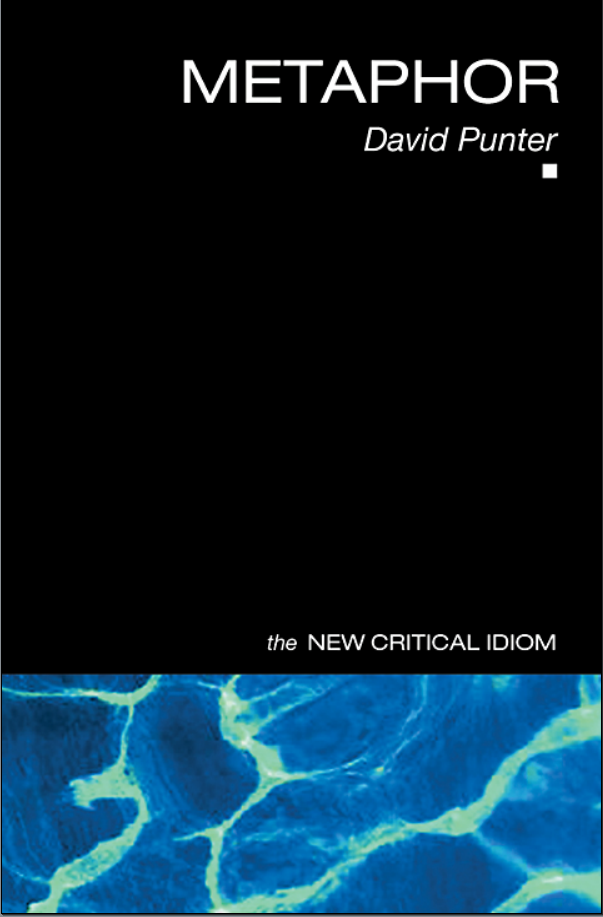
\includegraphics[width=0.24\textwidth]{./assets/negocio_metafora1.png}
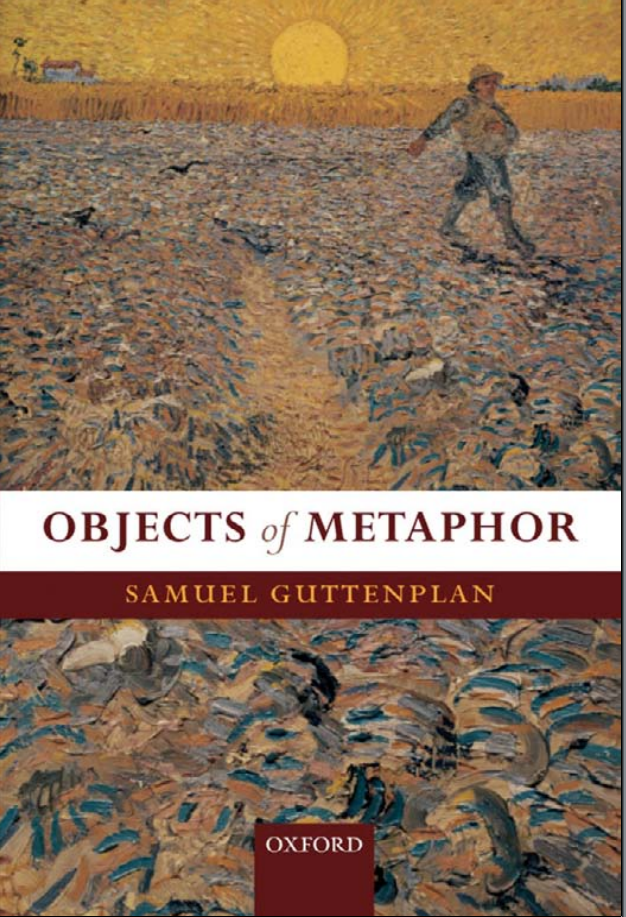
\includegraphics[width=0.24\textwidth]{./assets/negocio_metafora2.png}
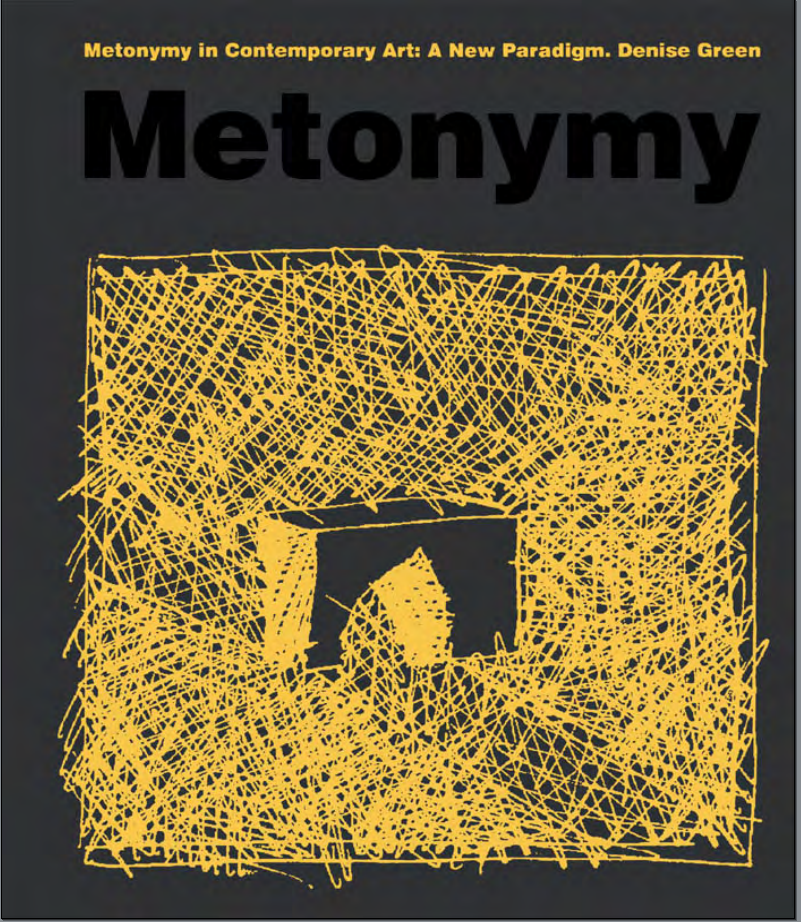
\includegraphics[width=0.24\textwidth]{./assets/negocio_metonimia1.png}
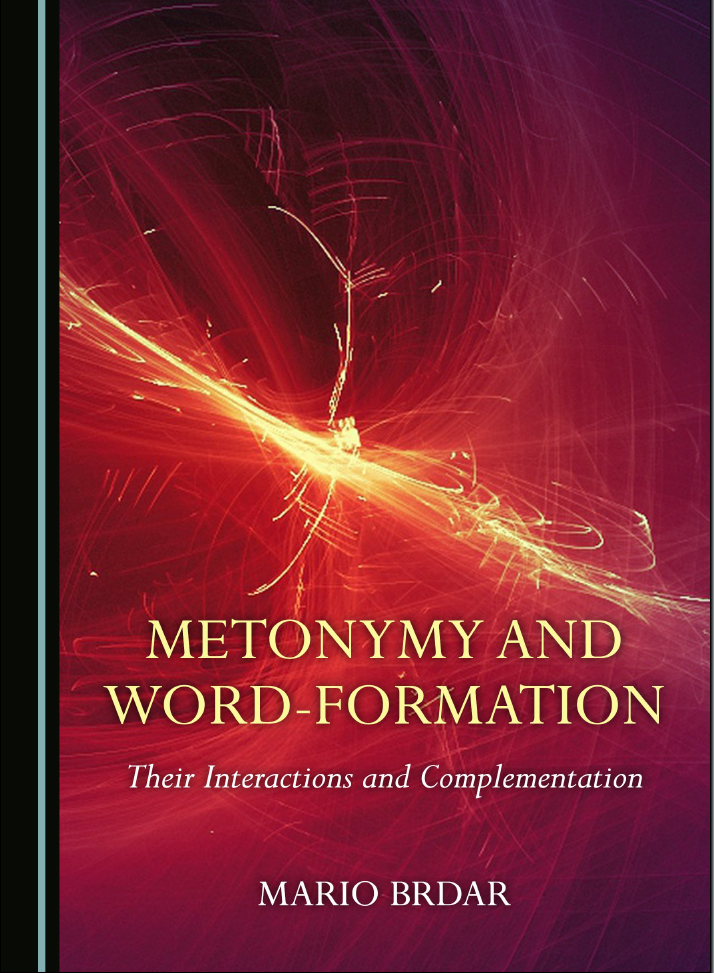
\includegraphics[width=0.24\textwidth]{./assets/negocio_metonimia2.png}
  \end{figure}
\end{frame}
\begin{frame}[label={sec:orga8c96b0}]{Ecuaciones}
\end{frame}
\begin{frame}[label={sec:org40e151a}]{Preparación de los datos}
\end{frame}
\begin{frame}[label={sec:org136279d}]{Despliegue}
\end{frame}


\section{Conclusiones}
\label{sec:org9321eac}

\bibliographystyle{ieeetr}
\bibliography{biblio} 
\end{document}